\documentclass[IJ]{cesj}
\usepackage{graphicx}
\usepackage{listings}

\author{Ga\"etan Lehmann}
\institute{Biologie du d\'eveloppement et de la reproduction, INRA de Jouy-en-Josas}

\title{Binary morphological closing and opening image filters}
\abstract{Binary morphological closing and opening image filters removes structures smaller than the structuring element in a binary image.}
\keyword{Morp}
\year{2005}

\leftmark{Ga\"etan Lehmann}
\rightmark{Ga\"etan Lehmann}

\begin{document}
\lstset{language=c++}
\maketitle
% \tableofcontents

\section{Description}
Binary morphological closing and opening image filters removes structures smaller than the structuring element in a binary image. Those filters also take care of boundary effects and of backgound values.

\section{Implementation}
BinaryMorphologicalClosingImageFilter and BinaryMorphologicalOpeningImageFilter are mainly a sequence of filters.

BinaryMorphologicalOpeningImageFilter runs a BinaryErodeImageFilter followed by a BinaryDilateImageFilter. Some background pixels may appear in the output image, so the user can choose the value of added background pixels.

BinaryMorphologicalClosingImageFilter runs a BinaryDilateImageFilter followed by a BinaryErodeImageFilter. If SafeBorder is true (the default), the BinaryDilateImageFilter is preceded by a ConstantPadImageFilter and the BinaryErodeImageFilter is followed by a CropImageFilter in order to avoid border effects. Finally, BinaryMorphologicalClosingImageFilter copy the background pixel from the input image to avoid the modifications of the background done by the BinaryErodeImageFilter. BinaryMorphologicalClosingImageFilter will never add backgound pixels so the backgound value used for the erode filter is automaticaly choosen.
\section{Example}

\begin{figure}[b]
\centering
\includegraphics[width=0.5\textwidth]{2th_cthead1.eps}
\caption{The input image. The image contains 3 pixels values: dark (0), dark grey (100) and light grey (200). All those values can be used as foreground value. In the next examples, the light grey is used as foreground and the other values as background.}
\end{figure}

\begin{figure}
\centering
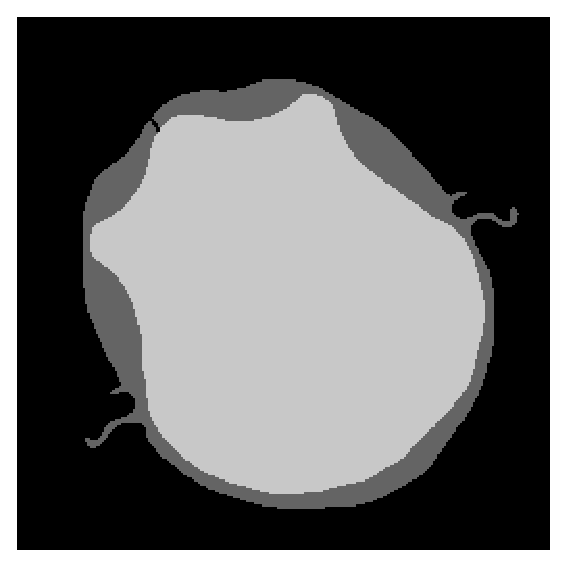
\includegraphics[width=0.5\textwidth]{close.eps}
\caption{The input image closed by a disc of radius 40, with SafeBorder=true. All background regions smaller than the structuring element are filled with the foreground value. The other background regions are not modified.}
\end{figure}

\begin{figure}
\centering
\includegraphics[width=0.5\textwidth]{close-unsafe.eps}
\caption{The closed image, with SafeBorder=false. The border effects are clearly visible on the right and on the bottom of the image, but are also there on the top and on the left of the image. SafeBorder=false must be used very carefully.}
\end{figure}

\begin{figure}
\centering
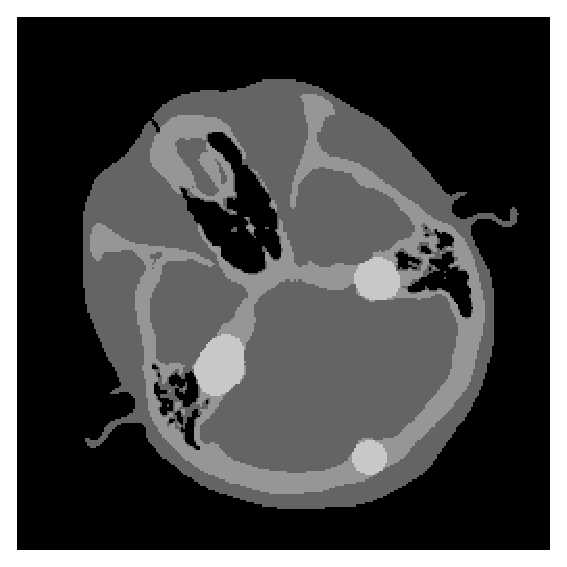
\includegraphics[width=0.5\textwidth]{open.eps}
\caption{The opened image with a disc of radius 8. Only the foreground (light grey) regions of the input image where the structuring element fit are kept in light grey; the other foreground regions are added to backgound (in middle grey (150)).}
\end{figure}

\end{document}
